\documentclass[sigconf,nonacm]{acmart}
\settopmatter{printacmref=false,printfolios=true}
\setcopyright{none}
\renewcommand\footnotetextcopyrightpermission[1]{}
\usepackage{amsmath,tabularx,array,enumitem,balance}
\definecolor{CourseBlue}{HTML}{315EFB}
\definecolor{CourseTeal}{HTML}{14877D}
\hypersetup{colorlinks=true,linkcolor=CourseBlue,citecolor=CourseTeal,urlcolor=CourseTeal}
\newcolumntype{Y}{>{\raggedright\arraybackslash}X}
\setlist{leftmargin=*,topsep=3pt,itemsep=2pt}
\newcommand{\CourseNumber}{COMSCI/ECON 206}
\newcommand{\CourseName}{Computational Microeconomics}
\newcommand{\CourseSession}{Autumn 2026 Session 1}
\newcommand{\Instructor}{Luyao Zhang}
\newcommand{\WorkshopSession}{Not specified}
\newcommand{\GitHubLink}{\href{https://github.com/Ceejay464/Adaptive_Sequencer_Selection}{Project repository}}
\newcommand{\TemplateRepository}{\url{https://github.com/sunshineluyao/ps1-overleaf-template}}
\newcommand{\ColabLink}{\href{https://colab.research.google.com/drive/140wnvKP6uoW_TY1fXSKdyZol7e7CtHf-}{Open Colab notebook}}
\newcommand{\DemoLink}{\url{https://huggingface.co/spaces/asdfxsasd/Sequencer_Selection_Mechanism_Design}}
\newcommand{\coursemeta}{\noindent\textbf{Submission to:} \CourseNumber{} --- \CourseName.\\
\textbf{Course session:} \CourseSession. \textbf{Workshop:} \WorkshopSession.\\
\textbf{Instructor:} \Instructor. \textbf{Assignment:} PS1 research proposal.\par\smallskip}
\title{Adaptive Sequencer Selection: Limiting Long-Run Concentration While Preserving Efficiency}
\author{Wang Zijie}
\affiliation{\institution{Duke Kunshan University}\city{Kunshan}\country{China}}
\renewcommand{\shortauthors}{Wang Zijie}

\begin{document}
\begin{teaserfigure}
\captionsetup{skip=8pt}
\centering
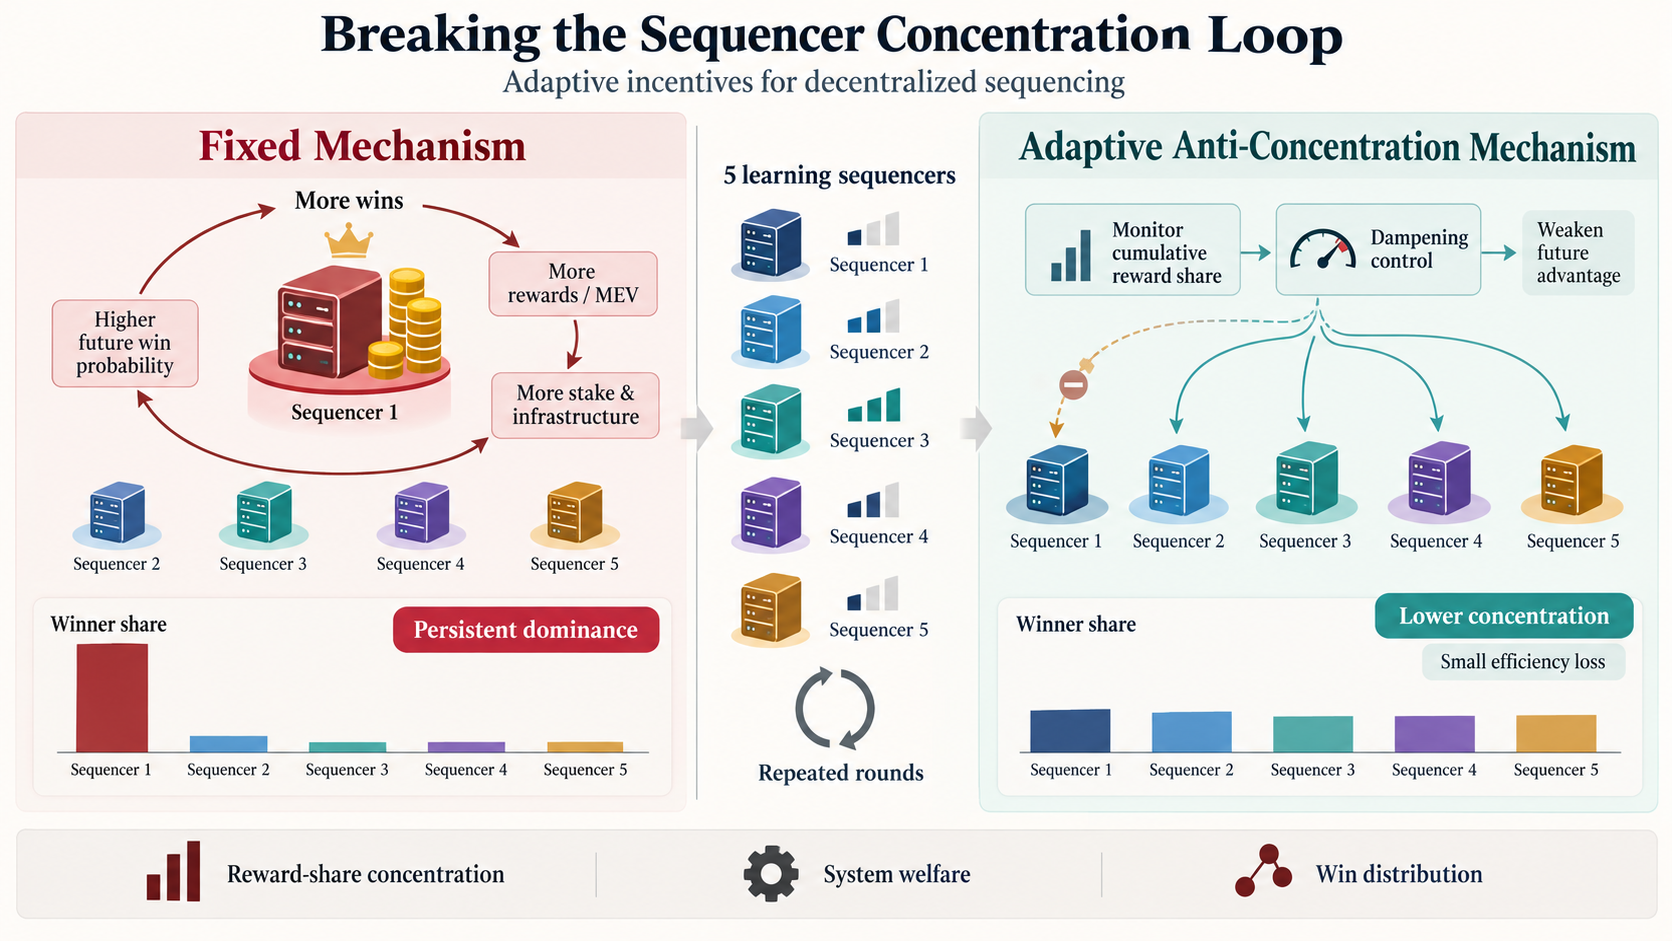
\includegraphics[width=\textwidth]{figures/sequencer_teaser_figure.png}
\caption{Proposed adaptive sequencer-selection experiment. Five self-interested learning sequencers repeatedly choose low, medium, or aggressive participation strategies. Their rewards, stake, and future selection chances create a possible positive-feedback loop. The adaptive mechanism weakens the future advantage of agents whose cumulative reward share becomes too large, and is evaluated against a fixed mechanism using concentration, welfare, and win-distribution outcomes.}
\Description{A diagram of five learning sequencers competing for transaction-ordering rights under fixed and adaptive mechanisms, with feedback from rewards and accumulated advantage to future selection probability.}
\label{fig:teaser}
\end{teaserfigure}
\maketitle\raggedbottom\coursemeta

\noindent\textcolor{CourseTeal}{\textbf{Proposal overview.}} This proposal studies whether an adaptive selection or reward rule can prevent persistent concentration among learning sequencers without sacrificing most of the system's efficiency. The planned client-side simulation compares a fixed benchmark with an anti-concentration mechanism across repeated competition among five agents.

\section{Three connected research questions}
Decentralized sequencer systems may re-centralize over time. Early winners can earn more fees and maximal extractable value (MEV), reinvest those gains in stake and infrastructure, and thereby increase their probability of winning future transaction-ordering rights. Existing mechanisms are often evaluated under fixed rules or static strategies, even though real sequencers can learn, reinvest, and adapt. The application considered here is repeated competition among five self-interested sequencers, each choosing a low, medium, or aggressive participation strategy in response to past rewards.

\noindent\textbf{Q1---Economics:} Can an adaptive sequencer-selection or reward rule reduce long-run concentration of sequencing power while preserving most system efficiency?\par
\noindent\textbf{Q2---Computation:} Can a multi-agent simulation measure how the adaptive mechanism changes concentration, welfare, and wins relative to the fixed mechanism?\par
\noindent\textbf{Q3---Behavior:} How do learning and reinvestment turn early reward differences into persistent dominance, and does adaptive feedback change the strategies agents learn?

The questions are interdependent. Incentive design defines the agents' rewards, learning determines their adaptive choices, and computation makes the resulting long-run distribution measurable. Figure~\ref{fig:teaser} summarizes this feedback loop and the proposed intervention.

\section{Answer to Q1: incentives and intellectual lineage}
The provisional hypothesis is that an adaptive rule can reduce persistent dominance with only a small loss in total welfare. The players are five sequencers. In every round, each selects a low, medium, or aggressive participation action using its experience of past rewards. Payoffs combine the reward from winning transaction-ordering rights with the consequences of the chosen participation level. Cumulative reward can improve future competitive position, creating an intertemporal incentive that a one-round benchmark does not capture.

The fixed mechanism is the economic benchmark: selection and rewards do not respond to accumulated concentration. The proposed adaptive rule weakens the future advantage of any sequencer whose cumulative reward share becomes too large. This comparison isolates the decentralization--efficiency trade-off. All findings in this proposal are planned or anticipated; no simulation result is presented as observed evidence.

\section{Answer to Q2: method and evaluation}
I plan to simulate five learning sequencers with multi-agent reinforcement learning. The common inputs are the three available participation strategies, the agents' reward histories, and the selection and reward rules. The baseline keeps the mechanism fixed. The treatment adds an adaptive anti-concentration adjustment that reduces the future advantage of agents once their cumulative reward share becomes disproportionately large.

The smallest feasible experiment runs both mechanisms from comparable initial conditions and records three outputs: reward-share concentration, total system welfare, and the distribution of sequencing wins across agents. Concentration can be summarized by the squared reward shares, $H=\sum_{i=1}^{5}s_i^2$, where $s_i$ is agent $i$'s cumulative reward share; lower values indicate a more even allocation. Welfare is the sum of agent rewards, and the win distribution shows whether apparent balance is persistent or merely temporary. Repeated seeds and identical evaluation horizons will provide a computational check. The game runs entirely in client-side JavaScript on the Hugging Face Static Space linked in the Open Science Statement. The anticipated result is lower persistent concentration with only a small welfare loss; this remains a hypothesis until the planned comparison is run.

\section{Answer to Q3: behavior and competing explanations}
The focal behavioral mechanism is adaptive reinforcement: agents repeat strategies that previously produced higher rewards, while accumulated rewards improve their future position. A competing explanation is that concentration arises mechanically from the selection rule even when strategies do not meaningfully adapt. The simulation can distinguish these explanations by comparing learning agents with otherwise identical agents following fixed strategies and by tracking whether strategy changes precede changes in reward share.

The adaptive mechanism changes the learning environment by reducing the value of exploiting an already dominant position. Evidence for the proposal would be a stable decline in concentration across repeated runs while welfare remains close to the fixed-mechanism benchmark. I would reconsider the mechanism if concentration quickly returns, if dominance simply rotates without becoming less persistent, or if the welfare loss is large. These simulated outcomes will describe the model rather than establish how human operators or deployed blockchain systems behave. A later test should vary learning rules, reinvestment strength, and information available to sequencers.


\section{Advanced development and future directions}
The longer-term objective is to explain and design against endogenous re-centralization in decentralized infrastructure. The enduring economic problem is how an institution can limit cumulative advantage without destroying incentives to participate efficiently. The computational problem is to evaluate rules when strategic agents learn rather than remain fixed. The behavioral problem is to understand how reward histories reshape future participation. Their integration makes it possible to study a policy whose effects emerge only through repeated feedback.

Future development will test alternative anti-concentration schedules, heterogeneous agents, longer horizons, and robustness to stronger reinvestment. The intellectual merit is an integrated account: behavioral science contributes adaptive behavior, economics contributes incentive design and the decentralization--efficiency trade-off, and computer science contributes the multi-agent simulation. Practically, the mechanism could help blockchain firms reduce dependence on dominant sequencers while preserving transaction performance. For the public sector, it offers a framework for more accountable decentralized infrastructure.

\begin{table}[h]\caption{From laureate foundations to a new interdisciplinary contribution.}
\begin{tabularx}{\columnwidth}{@{}p{1.6cm}Y@{}}\toprule
\textbf{Horizon}&\textbf{Milestone and evidence}\\\midrule
Foundation&Incentive design asks how institutional rules shape strategic behavior and welfare.\\
PS1&Five learning sequencers; fixed baseline; concentration, welfare, and win-distribution checks.\\
Next study&Adaptive anti-concentration design tested against fixed strategies and alternative learning rules.\\
Longer term&Robustness tests and validation in richer blockchain environments.\\
2056&Accountable decentralized infrastructure that limits cumulative advantage while retaining performance.\\\bottomrule
\end{tabularx}\end{table}

\noindent\textbf{Expected 2056 Nobel Prize and Turing Award contribution statement.}
By 2056, I aspire to contribute mechanism designs that keep decentralized infrastructure accountable as strategic participants learn and accumulate advantage. I will integrate economic incentive design, multi-agent computation, and adaptive behavior to advance the decentralization--efficiency frontier. Progress will be demonstrated by reproducible simulations, robust concentration and welfare evidence, and eventual validation in operational settings, with practical value for blockchain firms and public institutions.

\newpage

\subsection*{Open Science Statement}
\textbf{GitHub:} \GitHubLink\\
\textbf{Google Colab:} \ColabLink\par
The planned experiment uses synthetic agent histories and a client-side implementation. A public repository and verified Colab link have not yet been provided. The Hugging Face demonstration supplies the accessible interactive version described below.

\subsection*{Statement of Contribution to the UN's SDGs}
\textbf{Hugging Face:} \DemoLink\\
Through an open-access interactive simulation, this project aims to support \textbf{SDG 4---Quality Education}~\cite{sdg4} by helping students and practitioners explore how repeated rewards can concentrate sequencing power and how adaptive rules change that trajectory. Users can compare mechanisms in a web browser without server-side computation. Its educational usefulness remains to be evaluated.

\subsection*{Submission milestones}
The next milestones are to run repeated-seed comparisons, report the three proposed outcome families, test sensitivity to learning and reinvestment assumptions, and revise the mechanism if its welfare cost or residual concentration is too high. Appendix~\ref{app:abstract} records the current proposal map.

\clearpage\nobalance
\section*{Author Notes}
\subsection*{Acknowledgements}
This proposal was developed for COMSCI/ECON 206. No additional contributor information was provided. The author is responsible for the proposal and remaining errors.
\subsection*{Individual contribution}
The author formulated the research question, specified the fixed and adaptive mechanism comparison, designed the planned multi-agent experiment, and identified concentration, welfare, and win distribution as the principal outcomes.

\bibliographystyle{ACM-Reference-Format}\bibliography{references}
\appendix
\section{Technical details and reproducibility}
The planned model contains five agents and three actions per agent: low, medium, and aggressive participation. Each agent updates its behavior from past rewards. The fixed benchmark leaves selection and reward rules unchanged over time. The adaptive treatment reduces the future advantage of an agent when its cumulative reward share becomes too large. Planned outputs are the concentration index $H=\sum_{i=1}^{5}s_i^2$, total welfare, and agent-level win counts. Repeated random seeds, common horizons, and shared initial conditions will support comparison. The proposal does not yet claim completed experimental results.
\subsection{AI-use disclosure}
On September 19, 2026, Codex assisted in transferring the author's supplied proposal text into the provided Overleaf structure, adapting section-level prose, replacing the teaser figure, and checking PDF compilation and layout. The research idea, scenario, question, planned method, anticipated result, intellectual merits, and practical impacts were supplied by the author. The author remains responsible for every claim and computation.

\section{Cumulative Intellectual Development}
The proposal begins from the concern that decentralized sequencer systems may re-centralize through a feedback loop linking early rewards, reinvestment, and future selection probability. Its development turns that concern into a falsifiable comparison between a fixed mechanism and an adaptive rule. The central revision is conceptual: decentralization is treated as a dynamic outcome of learning and accumulated advantage rather than a static property of the initial allocation.

Appendix~\ref{app:abstract} summarizes the current proposal. Future versions should record simulation evidence and revisions separately from the anticipated findings stated here.

\section{Field and open-source inspiration}
The open-source inspiration is a browser-based simulation that makes a dynamic mechanism visible and testable without a server-side installation. The Hugging Face Static Space provides the application setting for comparing the fixed and adaptive rules. No field observations or photographs were supplied for this version, so none are claimed.

\section{Review response and revision record}
No peer-review record was supplied. The current version preserves the proposed strengths---a clear feedback mechanism, a concrete five-agent application, and measurable outcomes---while identifying open checks: repeated seeds, alternative learning rules, heterogeneous agents, and sensitivity to reinvestment strength. Future feedback and corresponding revisions should be recorded here.

\clearpage\onecolumn
\section{Structured abstract and cumulative proposal map}\label{app:abstract}
This table summarizes the current proposal and distinguishes planned evidence from anticipated results.
\par\medskip
\begin{table}[H]
\caption{Structured abstract and current proposal map.}
\label{tab:abstract-map}
\renewcommand{\arraystretch}{1.18}
\begin{tabularx}{\textwidth}{@{}p{0.27\textwidth}Y@{}}
\toprule
\textbf{Proposal element} & \textbf{Current statement / change} \\
\midrule
Background & Early sequencer winners may convert fees and MEV into stake, infrastructure, and a greater chance of future wins, causing re-centralization. \\
Motivation and application & Five self-interested sequencers repeatedly compete for transaction ordering and choose low, medium, or aggressive participation from past rewards. \\
Three connected questions & Can adaptive incentive design reduce concentration; can simulation measure the trade-off; and how do learning and reinvestment shape persistence? \\
Method and model assumptions & Multi-agent reinforcement learning compares a fixed mechanism with an adaptive rule that weakens excessive cumulative reward advantage. \\
Results or expected results & Planned measures are reward-share concentration, total welfare, and win distribution. The anticipated result is less persistent dominance with a small efficiency loss. \\
Intellectual merits & Economics supplies incentive design, computer science supplies simulation, and behavioral science supplies adaptive agents. \\
Practical impacts & Blockchain firms may reduce dominant-sequencer dependence; public institutions gain a framework for accountable infrastructure; learners gain an open web simulation. \\
Feedback received and revision made & No peer feedback was supplied. This version converts the proposal into the required five-section structure and labels all findings as planned or anticipated. \\
\bottomrule
\end{tabularx}
\end{table}
\noindent The current document distinguishes the supplied proposal, planned simulation evidence, and anticipated findings. Open-science links and the AI-use disclosure are reported above.

\end{document}
